\section{采食量预测模型:XGBoost}
\label{model}

\subsection{XGBoost模型简介}

\begin{figure*}
\begin{center}
	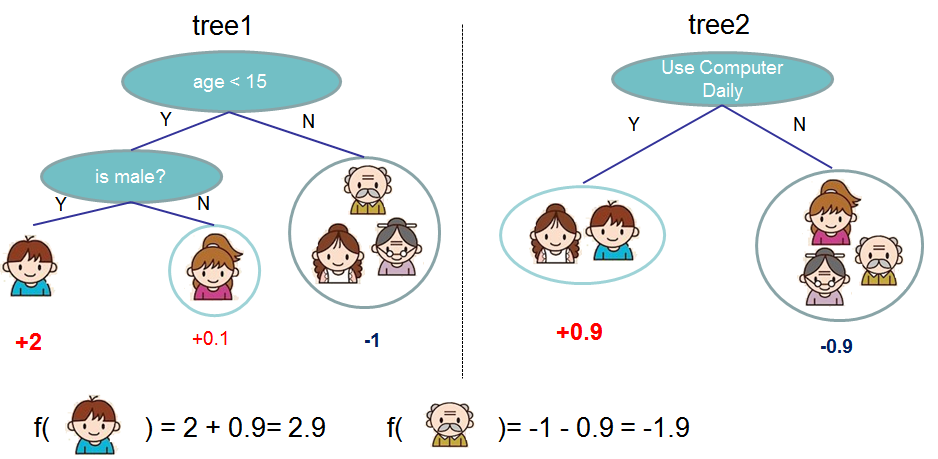
\includegraphics[width=0.8\linewidth]{twocart}
\caption{一个树集成的例子。该包含两棵树的模型解决分类问题,输入变量是每个人的年龄、性别、职业等特征,分类目标是“此人是否喜欢电脑游戏”。树集成将每棵树的输出结果组合起来(本例中为同权重地相加),例如小男孩分类结果为2.9,老爷爷分类结果为-1.9。如果我们设定模型分类阈值为0,则模型认为小男孩喜欢电脑游戏,老爷爷不喜欢。}
\label{twocart}
\end{center}
\end{figure*}


本工作采用XGBoost对采食量进行建模。XGBoost\cite{xgboost_github}是一个专注于梯度提升(gradient boost)算法的机器学习函数库,主要特点是具有优良的学习效果和高效的训练速度。该函数库诞生于2014年2月,最初由陈天奇博士设计、开发,论文\cite{Chen2016XGBoost}具体介绍了其实现原理和细节,演示文稿\cite{xgboost_slides}概述了其主要思想和算法原理。
仅在2015年,在Kaggle\cite{kaggle}竞赛中获胜的29个算法中,有17个使用了XGBoost库。在KDDCup 2015\cite{kddcup2015}竞赛中,排名前十的队伍全部使用了XGBoost库。

XGBoost用于解决监督学习(supervised learning)问题,在监督学习中模型利用训练集进行学习,以通过给定的量$x_i$(多个特征)来预测$y_i$。XGBoost是一种树集成(tree ensemble)模型\footnote{集成(ensemble)模型是一类组合多个性能相对弱的分类器/预测器实现强分类器/预测器的模型。所谓“三个臭皮匠赛过诸葛亮”。},即通过学习得到多棵树,组合起来解决分类问题或回归问题。
图\ref{twocart}展示了一个树集成的例子。

XGBoost优化的目标函数如式\ref{objf}所示:
\begin{equation}
\label{objf}
	obj = \sum_{i=1}^n l(y_i, \hat y_i^{(t)}) + \sum_{i=1}^t \Omega(f_i)
\end{equation}
其中$l(y_i, \hat y_i^{(t)})$表示模型对第$i$个训练集样本的预测误差(误差指标的定义根据问题的不同可以不同。
在回归问题中,均方误差MSE是常用的误差指标),$\Omega(f_i)$表示第$i$棵树的复杂度。
树的复杂度作为正则项,目的是为了控制模型的复杂程度,避免过复杂的模型过度拟合(overfit)训练集而缺乏泛化能力(对未见过样本的预测能力)。

在学习模型参数时,XGBoost采用相加策略:它递推地依次学习出各棵树,每次只增加一棵树,在学习第$t$棵树时,固定前$t-1$棵树不变,而用第$t$棵树去矫正前$t-1$棵树对于样本预测结果的误差(残差学习)。具体地,学习第$t$树时,优化目标函数$obj^{(t)}$为:
\begin{equation}
\label{objf_eachtree}
	obj^{(t)} = \sum_{i=1}^n l(y_i, \hat y_i^{(t-1)} + f_t(x_i)) + \Omega(f_t) + \textrm{常数}
\end{equation}

更多关于XGBoost算法细节请参考XGBoost网站文档、演示文稿和论文\cite{intro_xgboost, xgboost_slides,Chen2016XGBoost}。下面我们讨论使用XGBoost建模时需要重点考虑的模型参数。

\subsection{模型参数设置}

XGBoost的参数详解可参考\cite{xgboost_para}\footnote{XGBoost提供多种编程语言(Python, R, Java, Scala, C++)接口,该文档介绍R语言接口的参数,但其他语言参数与此基本相同。}。

\para{通用参数:}booster指定使用的booster(提升器),默认值为gbtree。使用默认值即可。
如想采用线性模型(采食量预测不适合采用线性模型),可以将其设为gblinear。

\para{Tree Booster参数:}
n\_estimator是树的个数,如需改善过拟合问题,可适当调小n\_estimator。
max\_depth是最大深度限制(模型最终构造的树可能不到此深度),如需改善过拟合问题,可适当调小max\_depth。由于当前预测采食量的模型使用输入变量很少,通常3-4层的树即足够。
eta是学习率,通常使用默认值即可,如需改善过拟合问题,可适当调小eta。
subsample和相关几个参数(colsample\_bytree、colsample\_bylevel)通过对训练集欠采样来避免模型欠拟合。当前预测采食量任务不需要欠采样。

其他参数一般不需要特别设置,使用默认值即可。

\subsection{最优参数搜索}
\label{best_para}

部分参数取值可以通过由在人为给定的参数空间中网格搜索(grid search,即暴力枚举每一种可能的参数组合)确定。
为了避免过拟合,在搜索每组参数组合时,可采用多折交叉验证。
本工作中如不特殊说明,我们采用8折交叉验证。

在实验中可以用Python的scikit-learn库中model\_selection包里的GridSearchCV类\cite{grid_search},它可便捷实现利用网格搜索和交叉验证确定最优参数组合。



